% smaller samples
\section{Analyzing Smaller Samples}
\label{sec:smallerDist}




We build a similar distribution using just 5 Tehsils (max) per province as seen in Figure~\ref{fig:fiveDist} with the code here:.
\begin{knitrout}
\definecolor{shadecolor}{rgb}{0.969, 0.969, 0.969}\color{fgcolor}\begin{kframe}
\begin{flushleft}
\ttfamily\noindent
\hlsymbol{pak5}{\ }\hlassignement{\usebox{\hlnormalsizeboxlessthan}-}{\ }\hlsymbol{pak}\hlkeyword{[}\hlsymbol{pak}\hlkeyword{\usebox{\hlnormalsizeboxdollar}}\hlsymbol{Tehsil}{\ }\hlkeyword{\usebox{\hlnormalsizeboxpercent}in\usebox{\hlnormalsizeboxpercent}}{\ }\hlfunctioncall{unlist}\hlkeyword{(}\hlfunctioncall{dlply}\hlkeyword{(}\hlsymbol{pak}\hlkeyword{,}{\ }\hlargument{.variables}{\ }\hlargument{=}{\ }\hlstring{"{}Province"{}}\hlkeyword{,}\hspace*{\fill}\\
\hlstd{}{\ }{\ }{\ }{\ }\hlargument{.fun}{\ }\hlargument{=}{\ }\hlsymbol{village.list}\hlkeyword{,}{\ }\hlargument{num}{\ }\hlargument{=}{\ }\hlnumber{5}\hlkeyword{,}{\ }\hlargument{unit}{\ }\hlargument{=}{\ }\hlstring{"{}Tehsil"{}}\hlkeyword{)}\hlkeyword{)}\hlkeyword{,}{\ }\hlkeyword{]}\hspace*{\fill}\\
\hlstd{}\hlsymbol{pak5}\hlkeyword{\usebox{\hlnormalsizeboxdollar}}\hlsymbol{Tehsil}{\ }\hlassignement{\usebox{\hlnormalsizeboxlessthan}-}{\ }\hlfunctioncall{factor}\hlkeyword{(}\hlsymbol{pak5}\hlkeyword{\usebox{\hlnormalsizeboxdollar}}\hlsymbol{Tehsil}\hlkeyword{)}\hspace*{\fill}\\
\hlstd{}\hlsymbol{rice5Perc}{\ }\hlassignement{\usebox{\hlnormalsizeboxlessthan}-}{\ }\hlfunctioncall{build.dist}\hlkeyword{(}\hlargument{data}{\ }\hlargument{=}{\ }\hlsymbol{pak5}\hlkeyword{,}{\ }\hlargument{lhs}{\ }\hlargument{=}{\ }\hlstring{"{}New\usebox{\hlnormalsizeboxunderscore}ID"{}}\hlkeyword{,}{\ }\hlargument{group}{\ }\hlargument{=}{\ }\hlstring{"{}Province"{}}\hlkeyword{,}\hspace*{\fill}\\
\hlstd{}{\ }{\ }{\ }{\ }\hlargument{question}{\ }\hlargument{=}{\ }\hlstring{"{}RiceLost"{}}\hlkeyword{)}\hspace*{\fill}\\
\hlstd{}\hlsymbol{rice5Perc}\hlkeyword{\usebox{\hlnormalsizeboxdollar}}\hlsymbol{Size}{\ }\hlassignement{\usebox{\hlnormalsizeboxlessthan}-}{\ }\hlstring{"{}5"{}}\hspace*{\fill}\\
\hlstd{}\hlsymbol{compare5}{\ }\hlassignement{\usebox{\hlnormalsizeboxlessthan}-}{\ }\hlfunctioncall{compare.dist}\hlkeyword{(}\hlsymbol{ricePerc}\hlkeyword{,}{\ }\hlsymbol{rice5Perc}\hlkeyword{,}{\ }\hlargument{by}{\ }\hlargument{=}{\ }\hlfunctioncall{c}\hlkeyword{(}\hlstring{"{}Province"{}}\hlkeyword{,}\hspace*{\fill}\\
\hlstd{}{\ }{\ }{\ }{\ }\hlstring{"{}RiceLost"{}}\hlkeyword{)}\hlkeyword{)}\hspace*{\fill}\\
\hlstd{}\hlsymbol{compare5}\hlkeyword{\usebox{\hlnormalsizeboxdollar}}\hlsymbol{Partial.Size}{\ }\hlassignement{\usebox{\hlnormalsizeboxlessthan}-}{\ }\hlfunctioncall{impute.col}\hlkeyword{(}\hlargument{col}{\ }\hlargument{=}{\ }\hlsymbol{compare5}\hlkeyword{\usebox{\hlnormalsizeboxdollar}}\hlsymbol{Partial.Size}\hlkeyword{,}\hspace*{\fill}\\
\hlstd{}{\ }{\ }{\ }{\ }\hlnumber{5}\hlkeyword{)}\hspace*{\fill}\\
\hlstd{}\hlfunctioncall{ggplot}\hlkeyword{(}\hlsymbol{rice5Perc}\hlkeyword{,}{\ }\hlfunctioncall{aes}\hlkeyword{(}\hlargument{x}{\ }\hlargument{=}{\ }\hlsymbol{RiceLost}\hlkeyword{,}{\ }\hlargument{y}{\ }\hlargument{=}{\ }\hlsymbol{Percent}\hlkeyword{)}\hlkeyword{)}{\ }\hlkeyword{+}{\ }\hlfunctioncall{geom\usebox{\hlnormalsizeboxunderscore}bar}\hlkeyword{(}\hlargument{stat}{\ }\hlargument{=}{\ }\hlstring{"{}identity"{}}\hlkeyword{)}{\ }\hlkeyword{+}\hspace*{\fill}\\
\hlstd{}{\ }{\ }{\ }{\ }\hlfunctioncall{facet\usebox{\hlnormalsizeboxunderscore}wrap}\hlkeyword{(}\hlkeyword{\urltilda{}}\hlsymbol{Province}\hlkeyword{)}{\ }\hlkeyword{+}{\ }\hlfunctioncall{opts}\hlkeyword{(}\hlargument{axis.text.x}{\ }\hlargument{=}{\ }\hlfunctioncall{theme\usebox{\hlnormalsizeboxunderscore}text}\hlkeyword{(}\hlargument{angle}{\ }\hlargument{=}{\ }\hlnumber{90}\hlkeyword{)}\hlkeyword{)}\mbox{}
\normalfont
\end{flushleft}
\end{kframe}
\end{knitrout}


\begin{figure}[!hbt]
\begin{knitrout}
\definecolor{shadecolor}{rgb}{0.969, 0.969, 0.969}\color{fgcolor}

{\centering 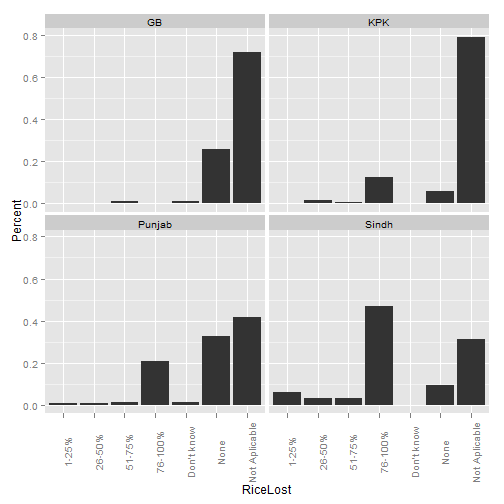
\includegraphics[width=.9\linewidth]{smallerDist/figures/fiveDistPlot} 

}


\end{knitrout}

\caption{Distribution for five Tehsils per Province.\label{fig:fiveDist}}
\end{figure}

The same distributions for 10 and 15 samples are seen in Figures~\ref{fig:tenDist} and \ref{fig:fifteenDist} respectively.  This time, for brevity, the code will not be displayed.

\begin{figure}[!hbt]
\begin{knitrout}
\definecolor{shadecolor}{rgb}{0.969, 0.969, 0.969}\color{fgcolor}

{\centering 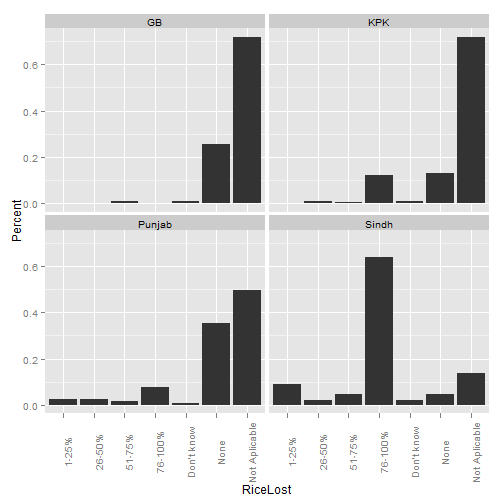
\includegraphics[width=.9\linewidth]{smallerDist/figures/tenDist} 

}


\end{knitrout}

\caption{Distribution for ten Tehsil per Province.\label{fig:tenDist}}
\end{figure}

\begin{figure}[!hbtp]
\begin{knitrout}
\definecolor{shadecolor}{rgb}{0.969, 0.969, 0.969}\color{fgcolor}

{\centering 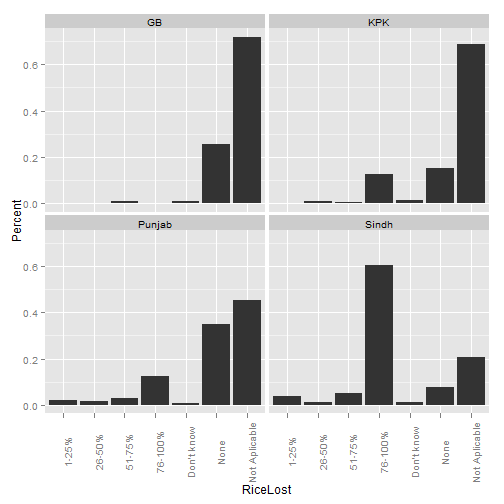
\includegraphics[width=.9\linewidth]{smallerDist/figures/fifteenDist} 

}


\end{knitrout}

\caption{Distribution for 15 Tehsils per Province.\label{fig:fifteenDist}}
\end{figure}

Now we wish to to look at the various distributions in a single plot.  Here is the code:
\begin{knitrout}
\definecolor{shadecolor}{rgb}{0.969, 0.969, 0.969}\color{fgcolor}\begin{kframe}
\begin{flushleft}
\ttfamily\noindent
\hlcomment{\usebox{\hlnormalsizeboxhash}{\ }plot{\ }distributions{\ }for{\ }all{\ }measurement{\ }sizes{\ }on{\ }same{\ }graph}\hspace*{\fill}\\
\hlstd{}\hlsymbol{allT}{\ }\hlassignement{\usebox{\hlnormalsizeboxlessthan}-}{\ }\hlfunctioncall{rbind}\hlkeyword{(}\hlsymbol{rice5Perc}\hlkeyword{,}{\ }\hlsymbol{rice10Perc}\hlkeyword{,}{\ }\hlsymbol{rice15Perc}\hlkeyword{,}{\ }\hlsymbol{ricePerc}\hlkeyword{)}\hspace*{\fill}\\
\hlstd{}\hlsymbol{allT}\hlkeyword{\usebox{\hlnormalsizeboxdollar}}\hlsymbol{Size}{\ }\hlassignement{\usebox{\hlnormalsizeboxlessthan}-}{\ }\hlfunctioncall{ordered}\hlkeyword{(}\hlsymbol{allT}\hlkeyword{\usebox{\hlnormalsizeboxdollar}}\hlsymbol{Size}\hlkeyword{,}{\ }\hlargument{levels}{\ }\hlargument{=}{\ }\hlfunctioncall{c}\hlkeyword{(}\hlnumber{5}\hlkeyword{,}{\ }\hlnumber{10}\hlkeyword{,}{\ }\hlnumber{15}\hlkeyword{,}{\ }\hlstring{"{}All"{}}\hlkeyword{)}\hlkeyword{)}\hspace*{\fill}\\
\hlstd{}\hlfunctioncall{ggplot}\hlkeyword{(}\hlsymbol{allT}\hlkeyword{,}{\ }\hlfunctioncall{aes}\hlkeyword{(}\hlargument{x}{\ }\hlargument{=}{\ }\hlsymbol{RiceLost}\hlkeyword{,}{\ }\hlargument{y}{\ }\hlargument{=}{\ }\hlsymbol{Percent}\hlkeyword{)}\hlkeyword{)}{\ }\hlkeyword{+}{\ }\hlfunctioncall{geom\usebox{\hlnormalsizeboxunderscore}bar}\hlkeyword{(}\hlfunctioncall{aes}\hlkeyword{(}\hlargument{group}{\ }\hlargument{=}{\ }\hlsymbol{Size}\hlkeyword{,}\hspace*{\fill}\\
\hlstd{}{\ }{\ }{\ }{\ }\hlargument{fill}{\ }\hlargument{=}{\ }\hlsymbol{Size}\hlkeyword{)}\hlkeyword{,}{\ }\hlargument{stat}{\ }\hlargument{=}{\ }\hlstring{"{}identity"{}}\hlkeyword{,}{\ }\hlargument{position}{\ }\hlargument{=}{\ }\hlstring{"{}dodge"{}}\hlkeyword{)}{\ }\hlkeyword{+}{\ }\hlfunctioncall{opts}\hlkeyword{(}\hlargument{axis.text.x}{\ }\hlargument{=}{\ }\hlfunctioncall{theme\usebox{\hlnormalsizeboxunderscore}text}\hlkeyword{(}\hlargument{angle}{\ }\hlargument{=}{\ }\hlnumber{90}\hlkeyword{)}\hlkeyword{)}{\ }\hlkeyword{+}\hspace*{\fill}\\
\hlstd{}{\ }{\ }{\ }{\ }\hlfunctioncall{facet\usebox{\hlnormalsizeboxunderscore}wrap}\hlkeyword{(}\hlkeyword{\urltilda{}}\hlsymbol{Province}\hlkeyword{)}\mbox{}
\normalfont
\end{flushleft}
\end{kframe}
\end{knitrout}


The plot is in Figure~\ref{fig:allDistInOne}.
\begin{figure}[!hbtp]
\begin{knitrout}
\definecolor{shadecolor}{rgb}{0.969, 0.969, 0.969}\color{fgcolor}

{\centering 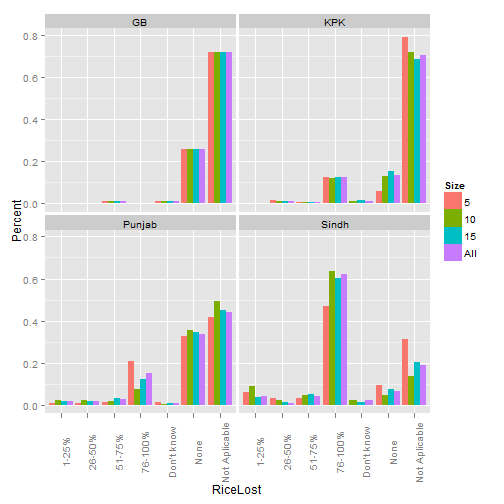
\includegraphics[width=.9\linewidth]{smallerDist/figures/allDistInOnePlot} 

}


\end{knitrout}

\caption{The distribution for all sampling types in one plot.\label{fig:allDistInOne}}
\end{figure}

Figure~\ref{fig:distErrors} displays the error between the smaller samples and the full distribution.  The code to do so is here:

\begin{knitrout}
\definecolor{shadecolor}{rgb}{0.969, 0.969, 0.969}\color{fgcolor}\begin{kframe}
\begin{flushleft}
\ttfamily\noindent
\hlsymbol{allC}{\ }\hlassignement{\usebox{\hlnormalsizeboxlessthan}-}{\ }\hlfunctioncall{rbind}\hlkeyword{(}\hlsymbol{compare5}\hlkeyword{,}{\ }\hlsymbol{compare10}\hlkeyword{,}{\ }\hlsymbol{compare15}\hlkeyword{)}\hspace*{\fill}\\
\hlstd{}\hlsymbol{allC}\hlkeyword{\usebox{\hlnormalsizeboxdollar}}\hlsymbol{Partial.Size}{\ }\hlassignement{\usebox{\hlnormalsizeboxlessthan}-}{\ }\hlfunctioncall{ordered}\hlkeyword{(}\hlsymbol{allC}\hlkeyword{\usebox{\hlnormalsizeboxdollar}}\hlsymbol{Partial.Size}\hlkeyword{,}{\ }\hlargument{levels}{\ }\hlargument{=}{\ }\hlfunctioncall{c}\hlkeyword{(}\hlnumber{5}\hlkeyword{,}{\ }\hlnumber{10}\hlkeyword{,}\hspace*{\fill}\\
\hlstd{}{\ }{\ }{\ }{\ }\hlnumber{15}\hlkeyword{)}\hlkeyword{)}\hspace*{\fill}\\
\hlstd{}\hlsymbol{allC}\hlkeyword{\usebox{\hlnormalsizeboxdollar}}\hlsymbol{Province}{\ }\hlassignement{\usebox{\hlnormalsizeboxlessthan}-}{\ }\hlfunctioncall{factor}\hlkeyword{(}\hlsymbol{allC}\hlkeyword{\usebox{\hlnormalsizeboxdollar}}\hlsymbol{Province}\hlkeyword{)}\hspace*{\fill}\\
\hlstd{}\hlfunctioncall{ggplot}\hlkeyword{(}\hlsymbol{allC}\hlkeyword{,}{\ }\hlfunctioncall{aes}\hlkeyword{(}\hlargument{x}{\ }\hlargument{=}{\ }\hlsymbol{RiceLost}\hlkeyword{,}{\ }\hlargument{y}{\ }\hlargument{=}{\ }\hlsymbol{.Diff}\hlkeyword{)}\hlkeyword{)}{\ }\hlkeyword{+}{\ }\hlfunctioncall{geom\usebox{\hlnormalsizeboxunderscore}line}\hlkeyword{(}\hlfunctioncall{aes}\hlkeyword{(}\hlargument{fill}{\ }\hlargument{=}{\ }\hlsymbol{Province}\hlkeyword{,}\hspace*{\fill}\\
\hlstd{}{\ }{\ }{\ }{\ }\hlargument{colour}{\ }\hlargument{=}{\ }\hlsymbol{Province}\hlkeyword{,}{\ }\hlargument{group}{\ }\hlargument{=}{\ }\hlsymbol{Province}\hlkeyword{)}\hlkeyword{)}{\ }\hlkeyword{+}{\ }\hlfunctioncall{opts}\hlkeyword{(}\hlargument{axis.text.x}{\ }\hlargument{=}{\ }\hlfunctioncall{theme\usebox{\hlnormalsizeboxunderscore}text}\hlkeyword{(}\hlargument{angle}{\ }\hlargument{=}{\ }\hlnumber{90}\hlkeyword{)}\hlkeyword{)}{\ }\hlkeyword{+}\hspace*{\fill}\\
\hlstd{}{\ }{\ }{\ }{\ }\hlfunctioncall{facet\usebox{\hlnormalsizeboxunderscore}wrap}\hlkeyword{(}\hlkeyword{\urltilda{}}\hlsymbol{Partial.Size}\hlkeyword{)}{\ }\hlkeyword{+}{\ }\hlfunctioncall{geom\usebox{\hlnormalsizeboxunderscore}hline}\hlkeyword{(}\hlargument{yintercept}{\ }\hlargument{=}{\ }\hlnumber{0}\hlkeyword{,}{\ }\hlargument{colour}{\ }\hlargument{=}{\ }\hlstring{"{}grey"{}}\hlkeyword{,}\hspace*{\fill}\\
\hlstd{}{\ }{\ }{\ }{\ }\hlargument{linetype}{\ }\hlargument{=}{\ }\hlnumber{2}\hlkeyword{)}\mbox{}
\normalfont
\end{flushleft}
\end{kframe}
\end{knitrout}


\begin{figure}[!hbtp]
\begin{knitrout}
\definecolor{shadecolor}{rgb}{0.969, 0.969, 0.969}\color{fgcolor}

{\centering 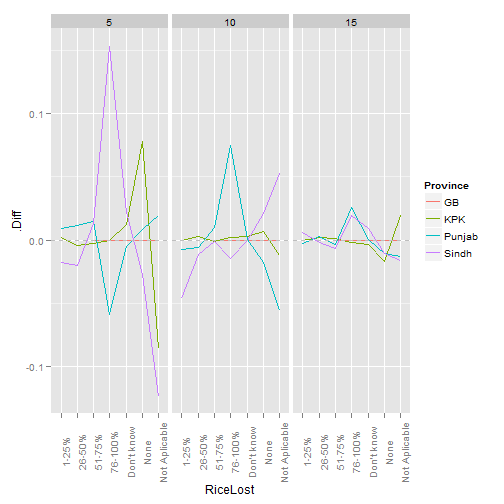
\includegraphics[width=.9\linewidth]{smallerDist/figures/distErrorsPlot} 

}


\end{knitrout}

\caption[Distribution Differences.]{The difference between the true distribution and the smaller smaples.\label{fig:distErrors}}
\end{figure}

Closing text.
